\documentclass[a4paper,12pt]{article}
\usepackage{mathrsfs}
\usepackage[utf8]{inputenc}
\usepackage[spanish]{babel}
\usepackage{amsmath}
\usepackage{amsfonts}
\usepackage{amssymb} 
\usepackage{graphicx} 
\usepackage{wrapfig}
\usepackage{enumitem}
\usepackage{fancyhdr}
\usepackage{float}
\usepackage{eurosym}
\usepackage{color}
\usepackage{circuitikz}
\usepackage{titling}
\usepackage{media9}
\usepackage{lipsum}
\usepackage{tocbibind}
\usepackage{listings}
\usepackage{tabularx}
\usepackage{tcolorbox}
\usepackage[table]{xcolor}
\usepackage{hyperref} 
\usepackage{bookmark}

\definecolor{lightblue}{RGB}{228, 244, 253}

\definecolor{dkgreen}{rgb}{0,0.6,0}
\definecolor{gray}{rgb}{0.5,0.5,0.5}
\definecolor{mauve}{rgb}{0.58,0,0.82}

\lstset{frame=tb,
  language=Python,
  inputencoding=utf8,
  extendedchars=true,
  aboveskip=3mm,
  belowskip=3mm,
  showstringspaces=false,
  columns=flexible,
  basicstyle={\small\ttfamily},
  numbers=none,
  numberstyle=\tiny\color{gray},
  keywordstyle=\color{blue},
  commentstyle=\color{dkgreen},
  stringstyle=\color{mauve},
  breaklines=true,
  breakatwhitespace=true,
  tabsize=3,
  literate=%
    {á}{{\'a}}1
    {é}{{\'e}}1
    {í}{{\'i}}1
    {ó}{{\'o}}1
    {ú}{{\'u}}1
    {ñ}{{\~n}}1
    {č}{{\v{c}}}1
}
\usepackage[left=3cm,right=3cm,top=3cm,bottom=4cm]{geometry}
\sloppy

% \pagestyle{fancy}
\providecommand{\abs}[1]{\lvert#1\rvert}
\providecommand{\norm}[1]{\lVert#1\rVert}

%%% Para las cabeceras
\newcommand{\hsp}{\hspace{20pt}}
\newcommand{\HRule}{\rule{\linewidth}{0.5mm}}
\headheight=50pt
%%% 
\newcommand{\vacio}{\textcolor{white}{ .}}

%%% Para que las ecuaciones se numeren
%%% con el número de sección y el de ecuación.
\renewcommand{\theequation}{\thesection.\arabic{equation}}


% Color azul para algunos 
% textos de la portada
\definecolor{azulportada}{rgb}{0.16, 0.32, 0.75}

%%%% Azul para textos de headings
\definecolor{azulinterior}{rgb}{0.0, 0.2, 0.6}

%%%%%%%%%%%%%%%%%%%%%%%%%%%%%%%%
%%%%%% Datos del proyecto %%%%%%
%%%%%%%%%%%%%%%%%%%%%%%%%%%%%%%%
%%%TÍTULO
%%% Escribirlo en minúsculas, el programa
%%% lo pondrá en mayúsculas en la portada.

\title{Aplicación de conceptos generales de RL }

%%%% AUTORES
\author{Lydia Ruiz Martínez \and Pablo Tuñón Laguna \and Alberto Velasco Rodríguez}

%%%%%%%%%%%%%%%%%%%%%
%%%%%%%%%%%%%%%%%%%%
\begin{document}

%%%%%%%%%%%%%%%%%%%%%%%%%%%%%%%
%%%%%%%%%%%%%%%%%%%%%%%%%%%%%%%
\begin{titlepage} %%%%% Aquí no hay que tocar nada.
	%%%% Las siguientes instrucciones generarán automáticamente
	%%%% la portada de tu proyecto.
	%%% Cambio de la estructura de esta página
\thispagestyle{empty}
\newgeometry{left=0.6cm,top=1.2cm,bottom=1.2cm}

\fbox{\parbox[c]{18.5cm}{
\begin{center}
\vspace{1.5cm}
{\fontfamily{ptm}\fontsize{24}{28.8}\selectfont{Universidad Pontificia Comillas}}\\
[3.5em]
{\fontfamily{ptm}\fontsize{24}{5}\selectfont{ICAI}}\\
[3em]
{\fontfamily{ptm}\fontsize{28}{5}\selectfont{CUADERNO DE TRABAJO}}\\
[1.5cm]
{\fontfamily{ptm}\fontsize{24}{5}\selectfont{Aprendizaje por refuerzo}}\\
[2cm]

% Autor del trabajo de investigación
\textcolor{azulportada}{\fontfamily{ptm}\fontsize{16}{5}\selectfont{\theauthor}}\\
[2cm]
% Título del trabajo
\textcolor{azulportada}
{\fontfamily{ptm}\fontsize{30}{5}\selectfont{\textsc{\thetitle}}}\\
%{\Huge\textbf{\thetitle}}\\
[1.2cm]

\includegraphics[width=8cm]{../fonts/Logo ICAI.png}
\\[1.8cm]

{\fontfamily{ptm}\fontsize{16}{5}\selectfont{Curso 2025-2026}}\\
[4cm]
\end{center}
}}
\restoregeometry
\end{titlepage}
 
 %%%% Volvemos a la estructura de la página normal

%%%%%%%%%%%%%%%%%%%%%%%%%%%%%%


%%%Encabezamiento y pie de página
%%% También se genera automáticamente
%%% Mejor no tocarlo mucho.
\renewcommand{\headrulewidth}{0.5pt}
\fancyhead[R]{
\textcolor{azulportada}{\fontfamily{ptm}\fontsize{10}{3}\selectfont{Proyecto final de Aprendizaje por refuerzo}}\\
{\fontfamily{ptm}\fontsize{10}{3}\selectfont{\theauthor}}}
\fancyhead[L]{
  \textcolor{azulinterior}{\fontfamily{ptm}\fontsize{14}{4}\selectfont{\textbf{\thetitle}}}\\
}

\pagestyle{fancy}

\renewcommand{\footrulewidth}{0.5pt}
\fancyfoot[L]{\footnotesize Universidad Pontificia de Comillas (ICAI) --- curso 2025-2026}
\fancyfoot[C]{\vacio}
\fancyfoot[R]{\footnotesize Página \thepage}

%%%%%%%%%%%%%%%%%%%%

\renewcommand{\contentsname}{Índice}
\addtocontents{toc}{\protect\setcounter{tocdepth}{-1}} % Quita el índice de la tabla de contenidos
\tableofcontents
\addtocontents{toc}{\protect\setcounter{tocdepth}{2}}

\newpage
\section{Navegación con tile coding}

Esta sección documenta el diseño, las decisiones y los resultados de la práctica de navegación con aproximación lineal y \textit{tile coding}. El objetivo es aprender una política que desplace al agente en un mapa de 10\,m por 10\,m hasta una zona objetivo evitando colisiones, usando acciones discretas de desplazamiento cardinal con paso de 0.25\,m. Se parte de una observación cruda $(x,y,\text{collision},\text{target})$ y se construye una representación dispersa mediante mosaicos solapados.

\subsection{Representación y generalización}
El estado continuo no se presta a una tabla de valores, así que se emplea \textit{tile coding} con varias rejillas solapadas. Cada rejilla activa exactamente un índice, por lo que el vector de entrada $\mathbf{x}(s)$ tiene exactamente $n_{\text{tilings}}$ unos y el resto ceros. La normalización por anchura y altura de tile desacopla la escala del mapa de la discretización. Se aplican desplazamientos distintos por rejilla con paso relativo $(3,1)$ en los ejes para romper alineamientos regulares y evitar patrones repetitivos que degradan la generalización. Con $n_{\text{tiles\_width}}=10$, $n_{\text{tiles\_height}}=10$ y $n_{\text{tilings}}=8$ se obtiene un compromiso útil: resolución suficiente en pasillos y solapamiento para transferir experiencia entre posiciones cercanas.

Los pesos se almacenan como una matriz $\texttt{weights}\in\mathbb{R}^{\texttt{num\_actions}\times\texttt{feature\_size}}$. Esta forma evita ambigüedades de indexado y permite sumar de manera vectorizada en las columnas correspondientes a los índices activos.

\subsection{Aproximación lineal e interpretación del gradiente}
Se aproxima $Q(s,a)$ con un modelo lineal por acción,
\[
Q(s,a)\approx \mathbf{w}_a^{\top}\mathbf{x}(s),
\]
donde $\mathbf{x}(s)$ es binaria y dispersa. La derivada de $Q$ respecto a $\mathbf{w}_a$ es exactamente $\mathbf{x}(s)$, así que el gradiente está implícito al actualizar únicamente las coordenadas activas. En cada transición se modifican $n_{\text{tilings}}$ pesos de la fila asociada a la acción ejecutada. Esto aconseja escalar la tasa de aprendizaje con el número de rejillas; como regla práctica, $\alpha\approx 0.1/n_{\text{tilings}}$ ofrece magnitudes razonables.

\subsection{Recompensa en \texttt{step()}: diseño, escala y riesgos}
El cálculo de la recompensa se integra en \texttt{step()} con tres casos:
\[
r=
\begin{cases}
+100, & \text{si el agente entra en la zona objetivo},\\
-100, & \text{si hay colisión},\\
- c - k\bigl(|x-c_x|+|y-c_y|\bigr), & \text{en otro caso},
\end{cases}
\]
donde $(c_x,c_y)$ es el centro de la zona objetivo. El término L1 genera una pendiente constante hacia la meta y evita efectos indeseados de la norma L2 (gradientes pequeños lejos del objetivo y posibles ganancias positivas al cuadrar). La escala de los extremos y del shaping es crítica: si los terminales son demasiado grandes dominan la señal y aparecen trayectorias absurdas; si $c$ y $k$ son demasiado pequeños, falta guía intermedia. Una horquilla inicial razonable es $c\in[0.05,0.1]$ y $k\in[0.005,0.02]$. Para atascos o colisiones sistemáticas se puede reducir $|100|$, subir $c$ para penalizar pasos inútiles o ajustar $k$ para hacer más pronunciada la pendiente.

Cuando una acción intenta cruzar una pared, conviene no mover la posición y terminar el episodio por colisión. La comprobación de llegada se hace sobre la posición efectiva tras validar colisiones.

\subsection{Funciones \texttt{get\_q\_values} y \texttt{update}}
\texttt{get\_q\_values} suma los pesos en los índices activos para cada acción. De forma vectorizada,
\[
\texttt{q\_values}=\texttt{weights}[:,\texttt{idx}].\texttt{sum(axis=1)}.
\]
En SARSA (semi-gradiente):
\[
\delta=\begin{cases}
r - Q(s,a), & \text{si termina},\\
r + \gamma Q(s',a') - Q(s,a), & \text{en otro caso},
\end{cases}
\quad
\mathbf{w}_a \leftarrow \mathbf{w}_a + \alpha\,\delta\,\mathbf{x}(s).
\]
En Q-learning se sustituye $Q(s',a')$ por $\max_{a'}Q(s',a')$. En ambos casos se actualizan solo las coordenadas activas.

\subsection{Exploración de $\epsilon$}
La política de comportamiento es $\epsilon$-greedy con decaimiento exponencial. Tres parámetros la gobiernan: fracción de episodios a partir de la cual empieza el decaimiento, razón de decaimiento y valor mínimo. Iniciar muy pronto o decaer agresivo cierra la exploración; iniciar muy tarde ralentiza la consolidación. En los ensayos fue equilibrado empezar entre el 50--70\% de episodios, con razón en $[0.95,0.99]$ y mínimo en $[0.02,0.05]$, de modo que al final la política sea casi determinista (como exige la evaluación).

\subsection{Parámetros}
Se fijaron $n_{\text{tiles\_width}}=10$, $n_{\text{tiles\_height}}=10$, $n_{\text{tilings}}=8$, zona objetivo $(2.5,8,1.0,2.0)$, $\gamma=0.99$ y $10{,}000$ episodios. Los hiperparámetros más sensibles fueron $\alpha$ y el calendario de $\epsilon$: un decaimiento excesivo degradó por cierre prematuro; posponer demasiado el inicio enlentece la convergencia. El refactor incluyó centralizar código, corregir la forma de \texttt{weights} a matriz bidimensional y exponer parámetros antes embebidos.

\subsection{Comparativa SARSA vs Q-learning}
Se entrenaron ambos agentes con los mismos mosaicos, $\gamma=0.99$, $10{,}000$ episodios, y un calendario de $\epsilon$ con decaimiento tardío. En este entorno determinista, Q-learning suele consolidar trayectorias más rápidas; SARSA tiende a políticas algo más conservadoras si hay estocasticidad. Las figuras siguientes muestran las métricas de cada agente:

\begin{figure}[H]
    \centering
    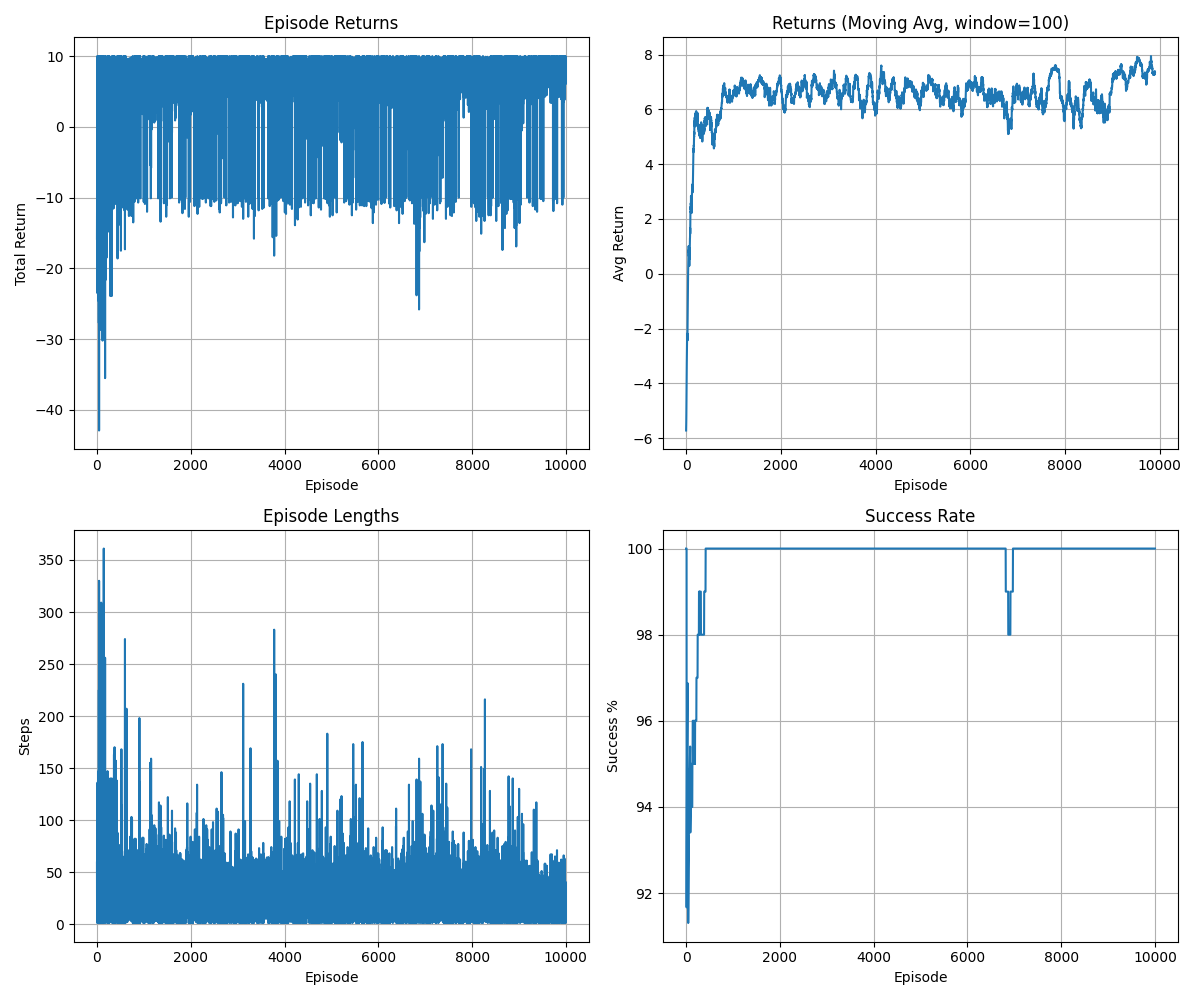
\includegraphics[width=\textwidth]{../plots/qlearning_metrics_10000_0.1_0.05_8.90.png}
    \caption{Q-learning: retornos, media móvil (100), longitudes y éxito.}
    \label{fig:qlearning-metrics}
\end{figure}

\begin{figure}[H]
    \centering
    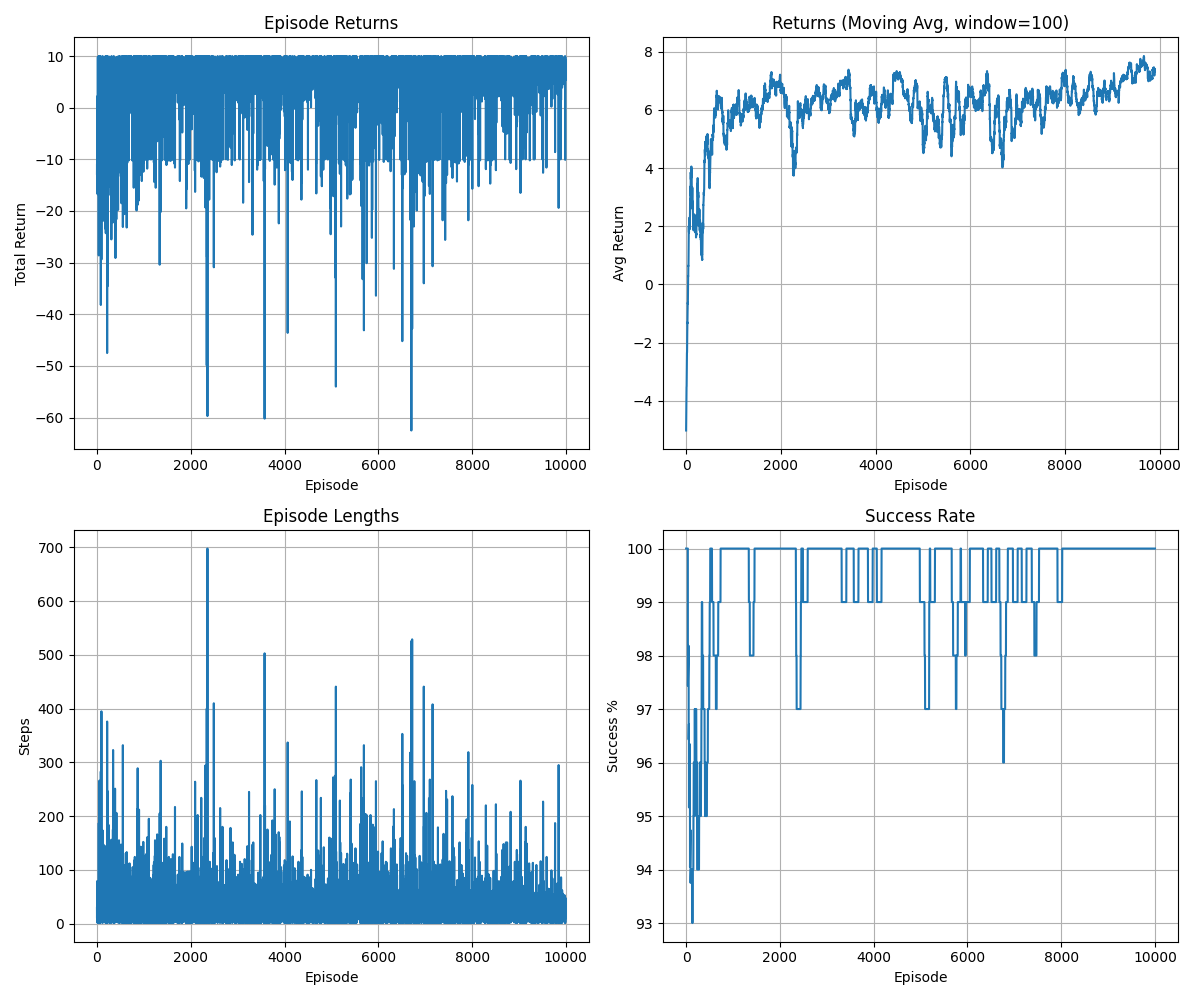
\includegraphics[width=\textwidth]{../plots/sarsa_metrics_10000_0.1_0.05_9.10.png}
    \caption{SARSA: retornos, media móvil (100), longitudes y éxito.}
    \label{fig:sarsa-metrics}
\end{figure}

En los resultados que obtuvimos, ambos alcanzan tasas de éxito muy altas. Q-learning tiende a converger algo más rápido en la media móvil y muestra longitudes medianas ligeramente menores en los últimos episodios; SARSA exhibe mayor variabilidad episódica pero una media móvil muy estable al final. Estas diferencias son coherentes con el objetivo temporal \emph{off-policy} de Q-learning frente a la naturaleza \emph{on-policy} de SARSA.

\newpage

\section{Operación en almacén}

\end{document}